\section{Modelling a metro system}
\label{metsys}

Reference will be made below to the various objects in the Zimulator
framework; the reader is referred to \Chapref{Chap:Zim} for
the meaning of these terms (e.g. \zobj{zbox}, \zobj{zpath}, \zobj{zlink}).

The terminology adopted here is `Metro System' and as mentioned above
this term is inexact. It is important to realize that not all metro
systems are identical, and source data for such systems may be
expressed in various ways. Therefore there is no single `correct' way
to construct a model of such a system, and the level of detail and precision
employed will vary depending on the model application and availability
of data.  In the present section will be discussed a reasonable way to
map a generic metro system to the ingredients available in the
Zimulator framework.

The system is deemed to have at least trains, stations, tracks and
passengers.  Beyond this minimum, there can be significant variation.

It is noted that while buses and the associated issues of more
extensive traffic modelling are complex and beyond the scope of this
discussion, buses travelling on dedicated or at least uncongested
traffic lanes might reasonably be interpreted as `trains' on
`tracks'. Buses in some cities are operated very much like trams or
streetcars.

Stations in some systems, like tram or LRT systems, are merely
platforms or sidewalks on which passengers may stand.  Some systems
have raised tracks and a station is thus comprised of a concourse with
platforms accessible via escalators or stairwells.  In subway systems,
a typical station is comprised of an underground concourse with
platforms at various extremedies, which concourse is accessible via a
set of tunnels leading from entrances, which might be independent, or
might connect to other structures like shopping malls or office
centres.  In some systems there are fare gates, through which
passengers walk on entry to the system; often passengers must also
pass through these when exiting. Sometimes these fare gates are part
of the station infrastructure; sometimes they are part of the vehicles
themselves.

In order that a comprehensive example be constructed below in \secref{Madrid},
here it is anticipated that a full station model will be employed.

At a high level, modelling of vehicle depots could be accomplished
within the present framework; nevertheless such modelling is
system-dependent and is not typically important from a passenger point
of view. Rather than maintain a conserved vehicle inventory via such
depot modelling, it will be seen to be sufficient to generate trains
at certain source points, and to discard these trains in sinks when
they have traversed their routes.

\subsection{Representation}
\label{sec:repr}

Objects in the system which are represented by \zobj{zboxen} are
trains, tracks, bounds, platforms, corridors, concourses, gates, `outgates'
and stations; each of these is a particular \zobj{ztype} as described in \secref{modparams} below.

A generic template for the construction of stations is shown in \Figref{fig:STN}.
\begin{figure}[ht]
  \centering
  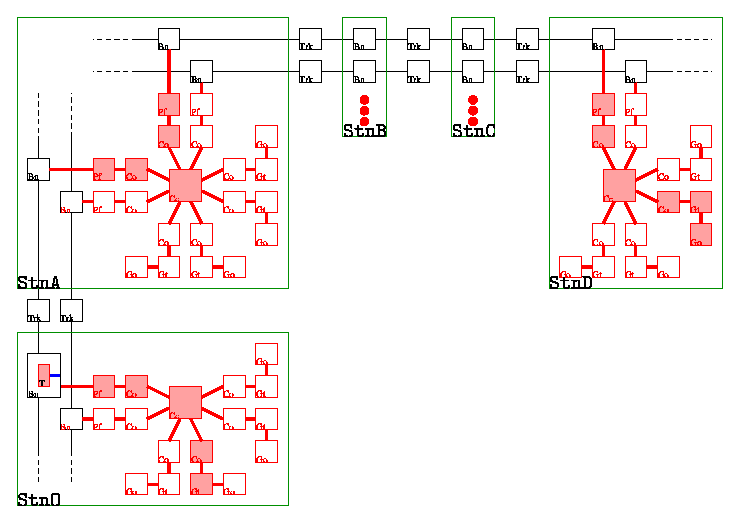
\includegraphics[angle=0,width=12cm]{60_figs/_SeveralStations2.eps}
  \caption{
    Five stations along sections of two transit lines:
    The red \zobj{zboxen} may contain passengers; the black may contain trains.
    \zobj{zlinks} which are red allow passengers; those which are black allow trains.
    The mnemonics {\tt Stn}, {\tt Pf}, {\tt Bn}, {\tt Co}, {\tt Cc}, {\tt Gt}, {\tt Go} and {\tt Trk} refer to a \zobj{zbox}
    representing a Station, Platform, Bound, Corridor, Concourse, Gate, `GateOut' and Track Segment, respectively.
    The blue \zobj{zlink} is an implied \zobj{zlink}, between the Train {\tt T} and Bound, and is traversable by passengers.
    The circular dots represent details not shown.
    \label{fig:STN}
  }
\end{figure}

Each train, represented by a \zobj{zbox}, is deployed on a \zobj{zpath} and
successively visits \zobj{zboxen} representing track intervals and representing bounds,
which are the stops next to platforms where passengers may board or alight.

Each passenger is also a \zobj{zbox}; a passenger is created via a
\zobj{zdemand} by copying a prototype passenger and placing the
\zobj{zbox} in a gate at the station of origin. A \zobj{zpath} is
assigned which controls the subsequent travel. The
passenger\footnote{As described in detail in the Zimulator
  documentation, visiting a \zobj{zbox} implies \emph{progression}
  through it, and moving to the next \zobj{zbox} involves
  \emph{shifting} to it via a \zobj{zlink}.}  successively visits
\zobj{zboxen} representing a gate, corridor, concourse, corridor and
platform, by traversing each and then shifting via \zobj{zlink} to the
next. The passenger then shifts to a train within the bound
\zobj{zbox} associated with the platform; this is made possible
by an implicit \zobj{zlink} from the train to the bound, traversible by passengers.
If later in the trip a transfer is to be undertaken, the passenger
shifts out to a platform, then to a corridor, concourse, corridor and
new platform at the transfer station, before shifting to a train in
the bound associated with the new platform. The passenger disembarks
by shifting out of the train to a platform, then eventually to a gate
and finally an `outgate' which is a sink via which the passenger quits
the system.

In this way, a passenger's full trip from station `O' to station `D' in the diagram
would involve visiting all the shaded \zobj{zboxen}.

The station construction displayed in \Figref{fig:STN} is general enough to
model many real-world stations.  Of course, some systems are
constructed such that common transfers may be made by simply walking
across a platform; this could be modeled, for example, by instead using
a simpler structure with a short corridor \zobj{zbox} between the platforms.

It is emphasized that correct interpretation of configurations like that shown in \Figref{fig:STN}
involves recognizing that time spent by a \zobj{zbox} occurs in \emph{progressing}
through various container \zobj{zboxen}, and not in instantaneous \emph{shifting}
from one to the next along \zobj{zlinks}.

\subsection{zsyntax files}
\label{seczsyn}

The data mentioned in the previous section are used to build the metro system using \zobj{zboxen}.
The metro system is thereby specified in the zsyntax files listed below.

Separation of zsyntax simulator input into particular files is entirely arbitrary;
the simulator is simply provided with zsyntax input, and it can be stored in one or
many files as seen fit by the user. 

\subsection{Simulator input files}

The simulator expects the system to be expressed in \zobj{zsyntax}.

There are several sets of information which must be expressed in order
to model the system; these include:
\begin{itemize}
\item The \zobj{zsystem} itself (a few global parameters)
\item A number of \zobj{ztypes} covering each kind of obejcts in the system to be modeled by a \zobj{zbox}
\item Static \zobj{zboxen} describing each metro station as in \Figref{fig:STN}
\item Static \zobj{zboxen} describing each track segment in the network.
\item Static \zobj{zlinks} describing connections of the track segments to the bounds at the stations.
\item Prototype \zobj{zboxen} from which trains and passengers are created.
\item \zobj{zpaths} which describe the paths through the system taken by each train line.
\item A number of \zobj{zschedules} which indicate the times for deployment of trains on paths.
\item A number of \zobj{zdemand} objects which describe passengers with intended destinations to be injected into the system.
\end{itemize}

In \Secref{modparams} below is described the mapping between metro-system parameters and the
individual attributes of Simulator objects like \zobj{zboxen}.

In the Madrid example in \Chapref{Chap:Metro}, the above list will be distributed among
six files which will be discussed in detail.

\subsection{System parameters}
\label{modparams}
The main concept in modelling a system is that progress of a
\zobj{zbox} through its container corresponds to progression of some
modeled degree of freedom. In the case of a Track \zobj{zbox}, the
position of the Train \zobj{zbox} inside is the spatial position of
the train on that section of track; in the case of a Bound
\zobj{zbox}, the progression simply corresponds to the time taken
while the train is waiting at a Bound (i.e.~dwelling time).

In this way most of the parameters associated with the metro system are expressed
as attributes of certain \zobj{ztypes}, and so are exhibited by the
various \zobj{zboxen} in the system.

Some of these parameters are shown and described below, by extracting
example pieces of zsyntax. Since these extracts are not in context,
the particular numerical values (e.g. {\tt L=1380} or {\tt S=100}) are
unimportant and are merely illustrative.

Model parameters represented in the {\tt Train} \zobj{ztype} include train capacity and train speed:
\begin{lstlisting}[mathescape]
  [ztype A=Train n=1 q=1 C={Pax 1} m=Bag l=30 L=1380 N=1380 S=0 $\chi$=<TrainDoors>
    v=20 R=S]
\end{lstlisting}
\begin{itemize}
\item {\tt m=Bag} -- Passengers need not traverse when contained in a train.
\item {\tt L=1380} or {\tt N=1380} -- controls the capacity of a
  train. If $L$ is used, then it is measured in the same units as {\tt Pax}.$l$.
  Train capacity could be determined via some kind of calibration, and will be discussed later.
\item {\tt v=20} -- Speed of a train. Length units match those of {\tt Track}.$L$, and $m/s$ are used here.
\item {\tt S=0} -- Space `between' passengers.
\end{itemize}

Model parameters represented in the {\tt Bound} \zobj{ztype} include dwelling time:
\begin{lstlisting}[mathescape]
  [ztype A=Bound n=1  m=Pipe C={Train 1} L=45 V=1 N=1]
\end{lstlisting}
\begin{itemize}
\item {\tt m=Pipe} -- Controls how trains may stop at a bound.
\item {\tt L=45} -- Controls how long a train stops at a bound, in conjunction with {\tt Train}.$v$ and {\tt Train}.$l$.
\item {\tt V=1} -- Limiting velocity for trains; this limits {\tt Train}.$v$.
\end{itemize}
The dwelling time in this example is 30 s; since the train has length 30, it can progress 15 out of 45 with limited velocity 1.

Model parameters represented in {\tt Track} include travel time between stations:
\begin{lstlisting}[mathescape]
  [ztype A=Track n=1 m=Pipe C={Train 1} L=1000 S=100]
\end{lstlisting}
\begin{itemize}
\item {\tt m=Pipe} -- Trains may not pass each other on a track.
\item {\tt L=1000} -- The distance between two subsequent stations. This is overridden in specific \zobj{zboxen} of this \zobj{ztype}.
\item {\tt S=100} -- Minimal distance between successive trains.
\end{itemize}

Model parameters represented in {\tt Concourse} and {\tt Corridor} include walking distances within stations:
\begin{lstlisting}[mathescape]
  [ztype A=Concourse n=1 m=Bag C={Pax 1} N=10000]
  [ztype A=Corridor n=1 m=Span C={Pax 1} L=200 W=10]
\end{lstlisting}  
\begin{itemize}
\item {\tt L=200 W=10} -- Capacity of a corridor will be 2000 passengers. The walking distance through is 200 m.
  These are overridden by each {\tt Co} \zobj{zbox}. In particular, $L$ could be determined via calibration.
\item {\tt N=10000} -- The capacity of the {\tt Concourse} is typically overestimated in order not to
  produce an artificial bottleneck in the system.
\end{itemize}
The walking \emph{times} within the system are then determined by passenger walking speeds, which
are specified either as an attribute of a prototype Passenger within a \zobj{zsource} inside
\zobj{zdemand}, or specified within the \zobj{zsource} as the parameters of a log-normal
distribution.

Model parameters represented in {\tt Platform}:
\begin{lstlisting}[mathescape]
  [ztype A=Platform n=1 m=Bag C={Pax 1} L=4000]
\end{lstlisting}
\begin{itemize}
\item {\tt m=Bag} -- Passengers do not traverse a platform; they simply wait there.
\item {\tt L=4000} -- Capacity of a platform. This is not usually important for simulation, unless there is special interest in saturation of platforms.
\end{itemize}

The \zobj{ztypes} of {\tt Gate} and {\tt Platform} have a containment type of `Bag', thereby having only capacity
but no traversal attributes.

%\subsection{Simulation output}
%...

\subsection{Calibration}

In very general terms, there may be `ground truth' sources of data
which can be used to calibrate aspects of the simulation. For example,
there may be sensors on train platforms which can be used to calibrate
[effective] train speeds. There may be a farecard system which records
the precise times of passengers `tapping' in an out of the system;
this could be used to calibrate not only train speeds but also walking
times within the system and possibly other properties like effective
train capacities.

In section \secref{Chap:MadCali} an illustrative example of such
calibration will be given, calibrating the two-parameters of the
log-normal distribution used for passenger walking speeds.  Although
the system approximately modeled is a real-world system, the
`ground-truth' data utilised will be synthetic.
